\chapter{Zusammenfassung \& Fazit}\label{chap:zusammenfassung-und-fazit}

Nachdem wir nun die letzten Wochen und Monate mit der Entwicklung der Anwendung verbracht haben, schließen wir das Projekt ab. Wir haben viele Dinge gelernt, uns mit neuen Konzepten befasst und eine neue Programmiersprache gelernt. Aber wir haben uns auch mit einigen teils hartnäckigen Problemen auseinandersetzen müssen, die uns Zeit und Nerven gekostet haben und dazu geführt haben, dass wir nicht alles wie geplant umsetzen konnten.

\section{Reflexion des Vorgehens}\label{sec:reflexion}
\subsection{Aufgabenteilung}
Wir haben uns direkt zu Beginn des Semesters bei unserem Dozenten um das Thema beworben, ohne, dass dieses ausgeschrieben war. Der Hintergrund war, dass wir die Thematik, die Visualisierung eines Algorithmus' interessant fanden, aber auch die Programmiersprache Scala hatte ihren Reiz.

Nachdem wir die Zusage bekamen, richtete Herr Kerst ein git-Repository\footnote{\url{https://github.com/TobsCore/Visual-Mergesort/}} auf github ein und erstellte dort eine Vorlage für diese Dokumentation, die in \LaTeX geschrieben sein sollte. Außerdem wurde das eigentliche Scala Projekt eingerichtet, also die Ordner-Struktur und die Entwicklungsumgebung \texttt{IntelliJ IDEA}. Da wir uns entschieden, \texttt{sbt} als Build Tool und für das Verwalten von \textit{Dependencies} zu verwenden, wurde schon früh die \texttt{build.sbt} Datei erstellt und mit den nötigsten Informationen befüllt, sodass man ein Programm mit Scala kompilieren konnte.

Nachdem diese Vorbereitungen getroffen waren, lasen wir uns intensiv in die Sprache ein. Hierbei ging es nicht nur darum, die Syntax zu verstehen und anwenden zu können, sondern auch die in der Sprache üblichen \texttt{Code Conventions} kennenzulernen und uns mit der funktionalen Programmierung etwas näher auseinanderzusetzen. Das spiegelt sich zum Beispiel darin wieder, dass wir probiert haben, nur \texttt{val}--Values zu benutzen, anstelle von möglicherweise \texttt{var}iablen Werten. Auch die Schleifen sind häufig ohne direkte Zählvariable, sondern mit \texttt{zipWithIndex} geschrieben worden und wir nutzten auch sonst viele Scala Features. Ganz besonders zu erwähnen seien hier \texttt{Pattern Matching} und der (quasi ternäre) \texttt{ternäre if}--Operator.

Die Programmiersprache Scala zu lernen hat zwar viel Zeit in Anspruch genommen, doch hat uns im Endeffekt sehr geholfen, da wir uns nicht mit elementaren Syntax-Problemen auseinander setzen mussten, sondern uns bei der Entwicklung auf die wesentlichen Probleme beschränken konnten.

\subsubsection{Unser Test--Programm}
Wir haben die Entwicklung mit einer anderen Anwendung begonnen, die nichts mit der eigentlichen Projektarbeit zu tun hatte. Wir haben uns dafür entschieden, damit wir uns gemeinsam an die Scala Syntax gewöhnen und wir wollten dadurch ein besseres Verständnis von ScalaFX erlangen. Die Test-Anwendung hat den User dazu aufgefordert eine Zahl in ein Textfeld einzugeben und hat dann der Eingabe entsprechend viele Balken auf einen \texttt{Canvas} gezeichnet. Dies war bereits eine wichtige Entscheidung, da wir hierbei merkten, dass man die Elemente auf einer \texttt{Canvas} nicht ausreichend manipulieren kann und wir uns somit für eine \texttt{Pane} als \textit{Zeichenfläche} entschieden.

\begin{figure}[!htb]
    \centering
      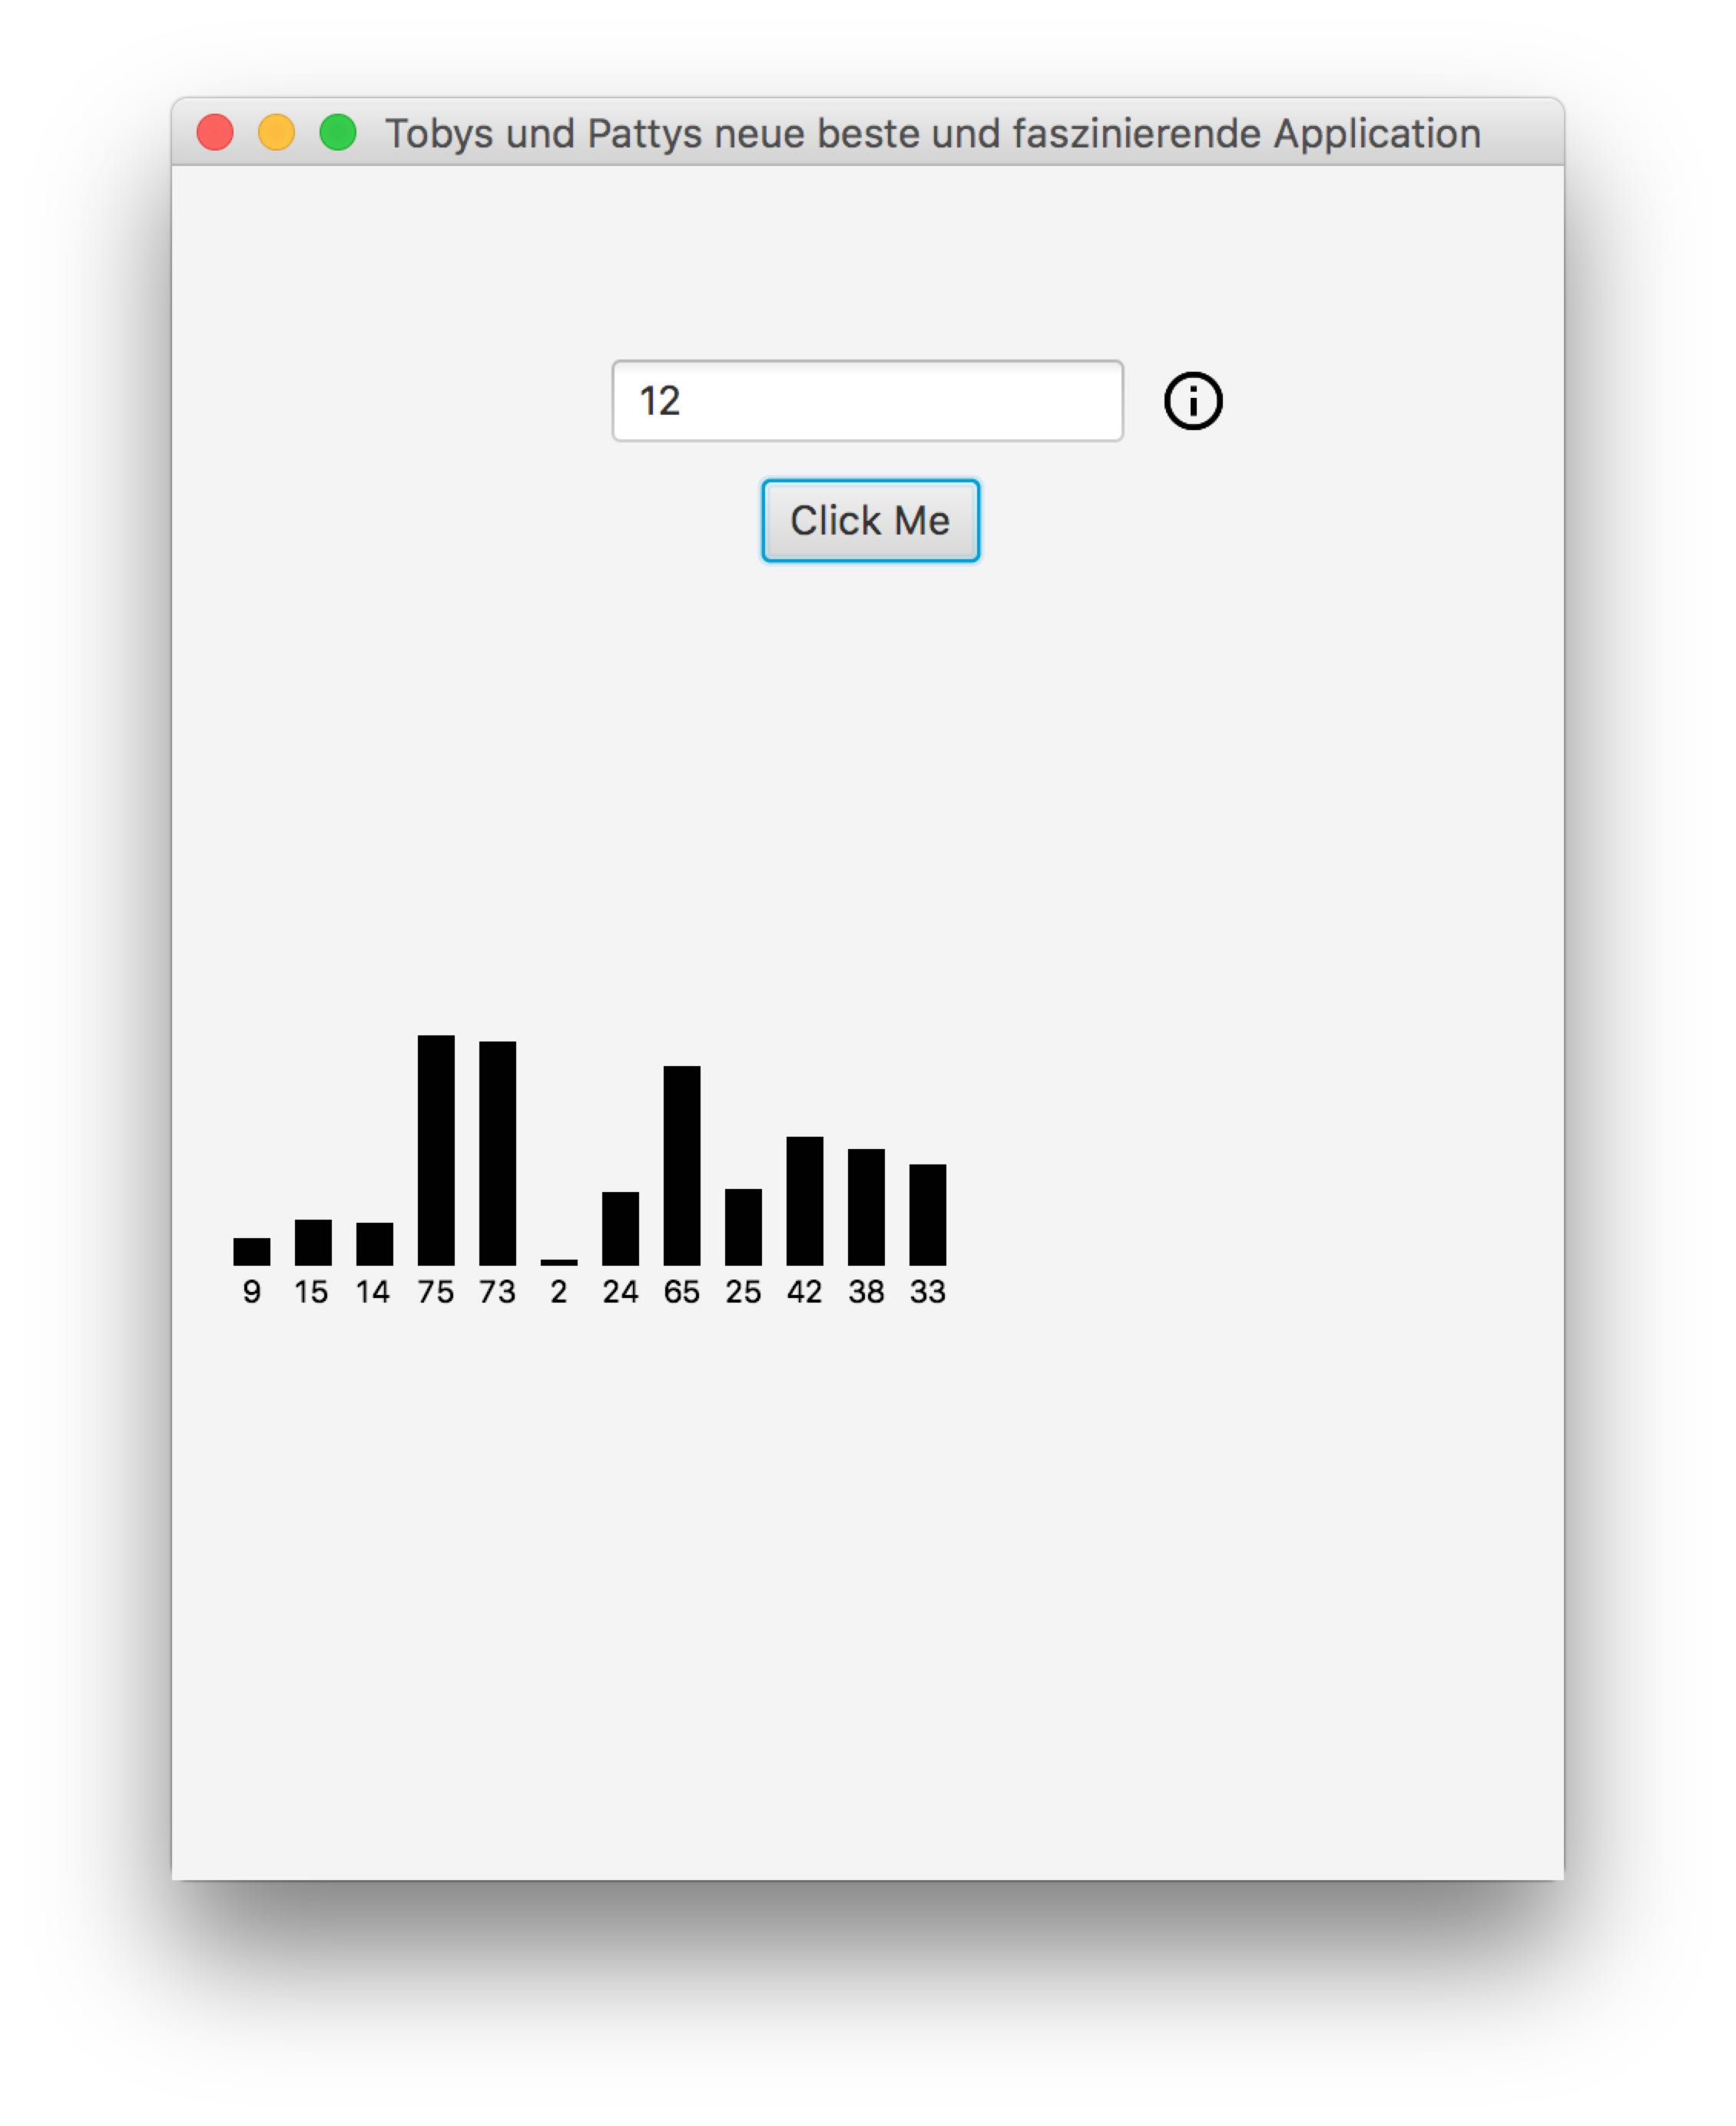
\includegraphics[width=0.55\linewidth]{test-anwendung1}
    \caption{Test Anwendung: Generierung der Balken}
\end{figure}

Außerdem war es eine gute Entscheidung, dass wir uns erst mit einer Anwendung beschäftigten, bei der wir viele Fehler machen konnten, da wir somit keine Design-Entscheidungen im späteren Verlauf bereuen würden.


Das Resultat ist, dass wir selbstbewusst die Beispielanwendung löschten und uns mit einem ausreichend guten Vorwissen an die Entwicklung der eigentlichen Aufgabe machten. Wir wussten nun, wie man auf Events reagiert, wie man Elemente in FXML definiert und in dem Controller anspricht. Wir konnten Elemente nun manipulieren (zwar auf einem \texttt{Canvas}) und kannten uns nun besser mit der baumartigen Struktur von JavaFX aus, bei der oben die \texttt{Stage}, darunter die \texttt{Scene} und darunter die \texttt{Node}s waren.


\begin{figure}[!htb]
    \centering
      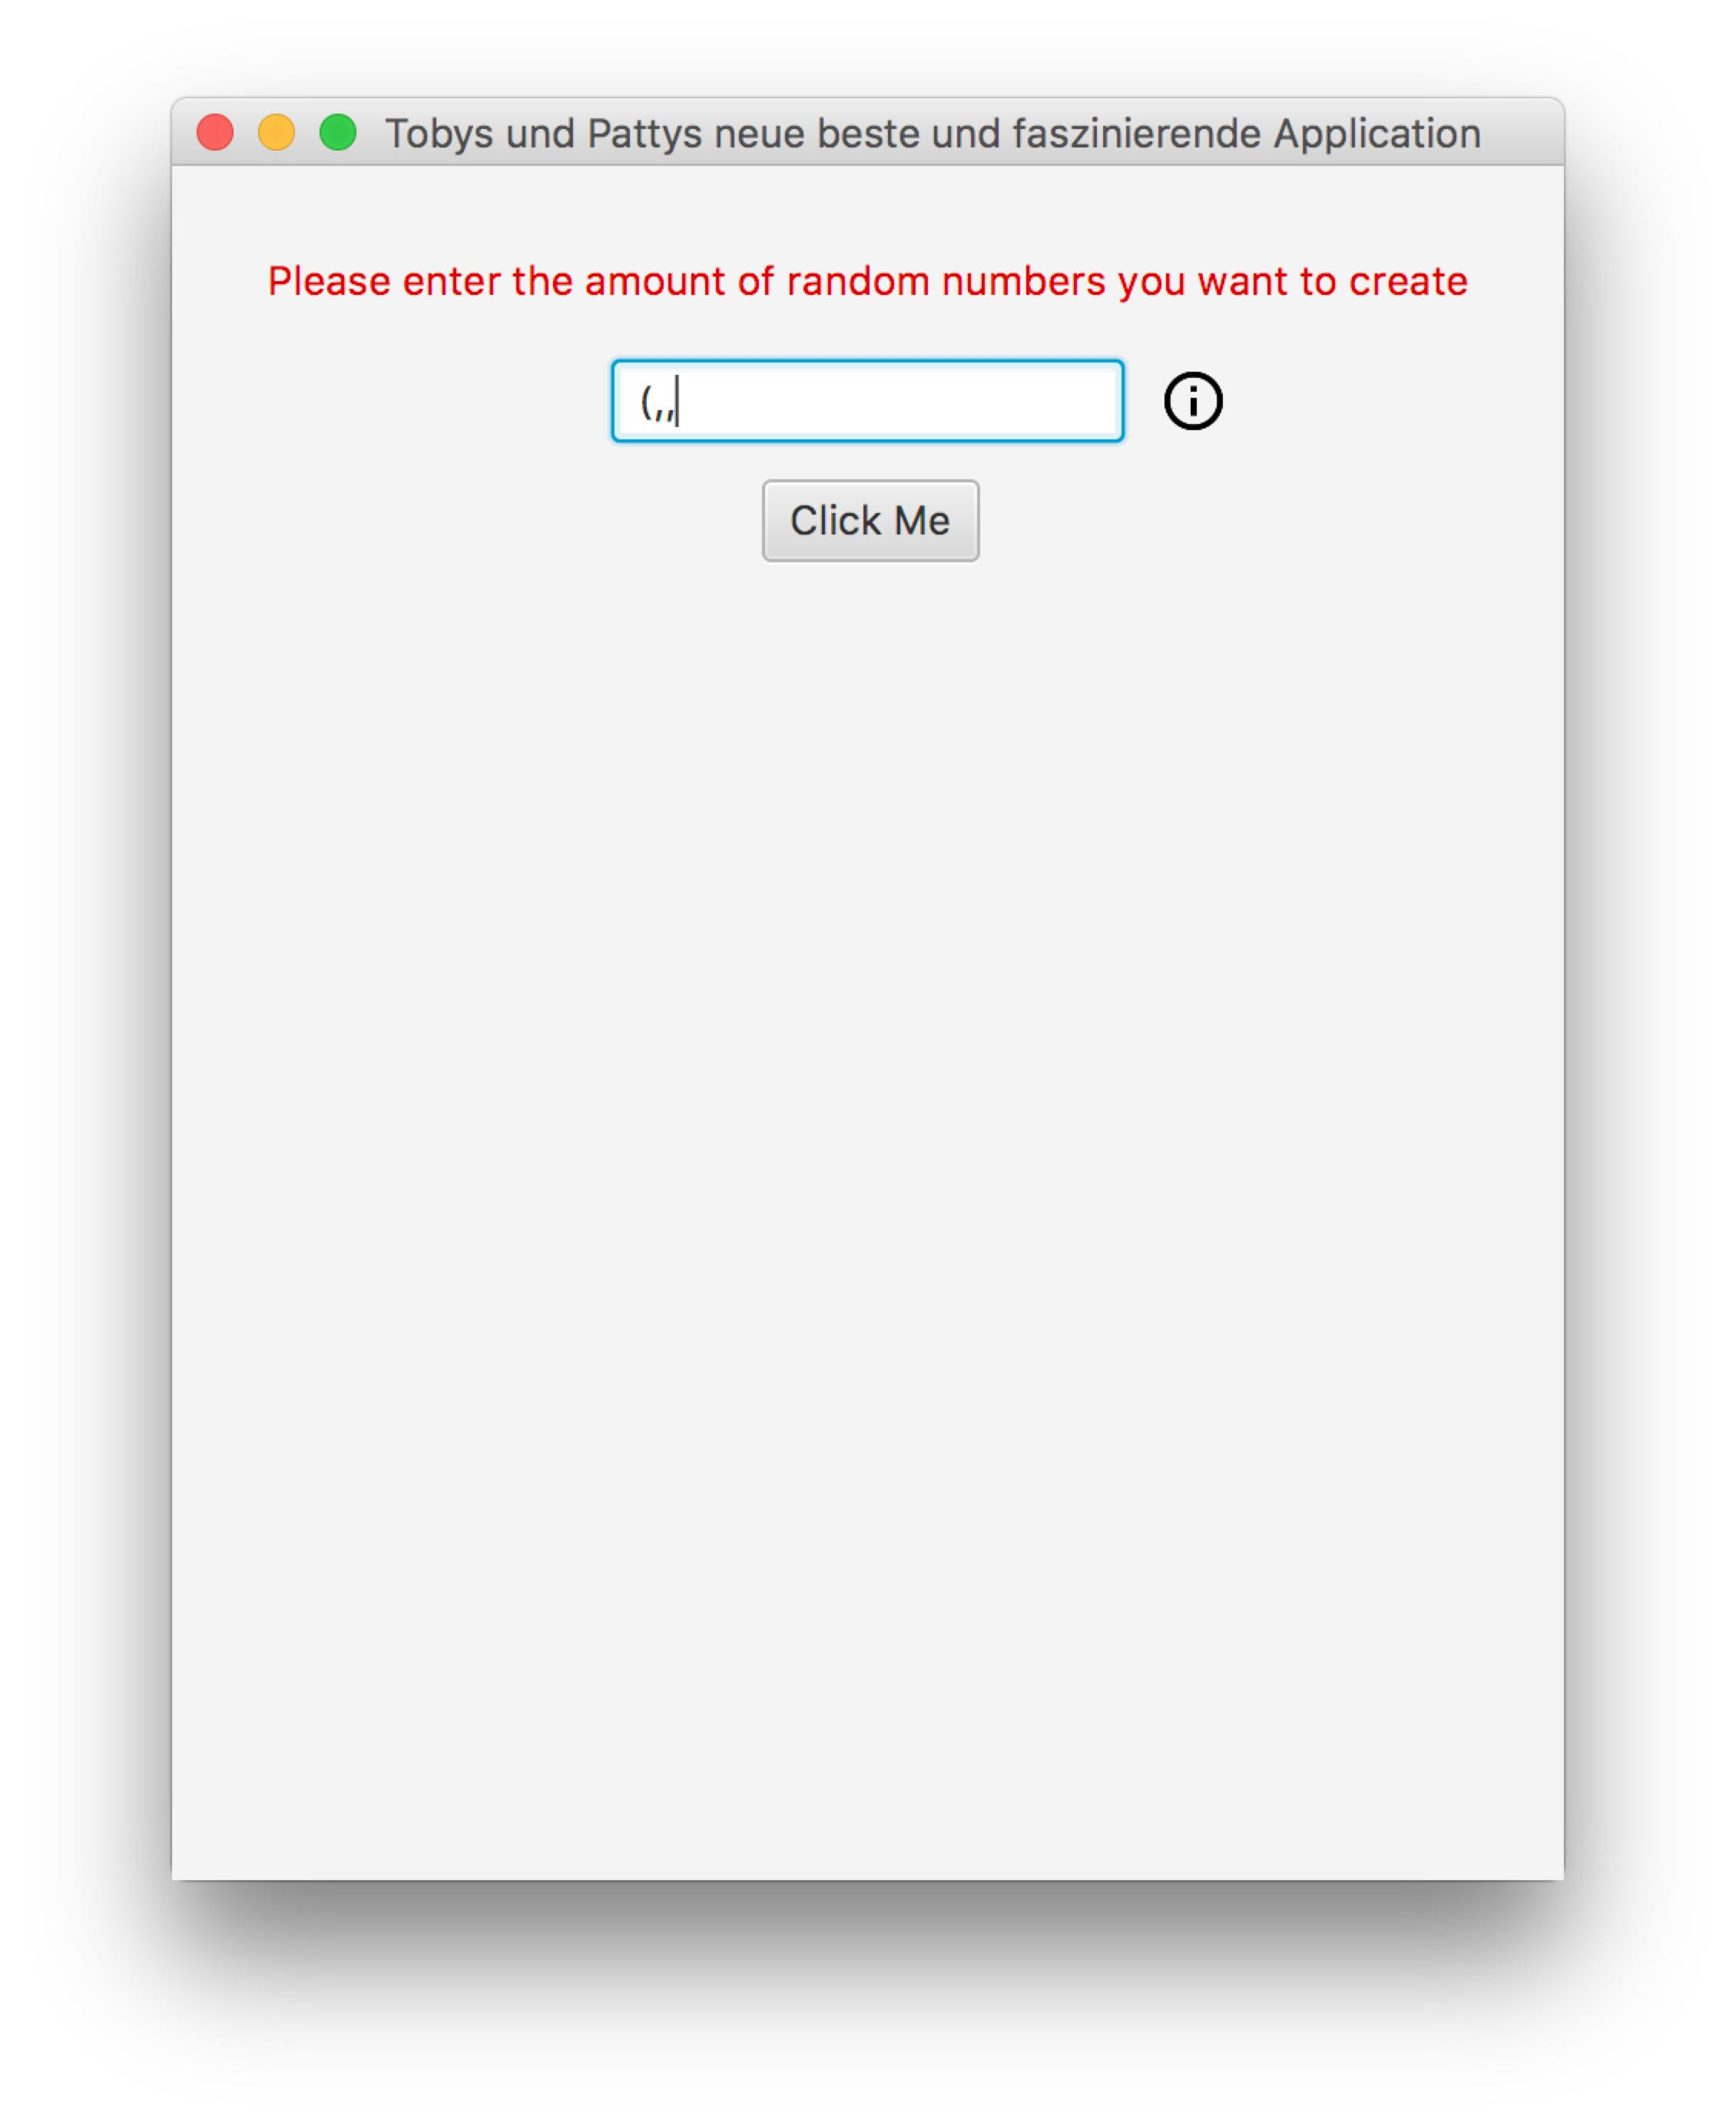
\includegraphics[width=0.55\linewidth]{test-anwendung2}
    \caption{Test Anwendung: Fehlermeldung bei Falscheingabe}
\end{figure}

\subsubsection{Gemeinsame Entwicklung}
Danach haben wir uns täglich getroffen und gemeinsam an der Anwendung gearbeitet. Hierbei haben wir die meiste Zeit vor einem Bildschirm gesessen und gemeinsam entwickelt. Dies hat sich als sehr sinnvoll herausgestellt, da man so schneller Fehlern vorbeugen konnte und wir kleine Probleme diskutieren konnten, ohne den anderen aus Gedanken reißen zu müssen, was eher passiert, wenn jeder an seinem Teil entwickelt. Somit nutzten wir die ganzen Vorteile von \textit{Pair Programming}\footnote{\url{https://www.agilealliance.org/glossary/pairing/}}

\begin{itemize}
\item Wir haben besseren Code geschrieben
\item Wir kannten alle Code-Teile und konnten so Bugs schneller finden und fixen
\item Wir haben viel diskutieren können
\end{itemize}

Im späteren Verlauf wurden einzelne Teile vermehrt aufgeteilt, da es sich hierbei um \textit{einfach zu schreibenden} Code handelte oder weil es zeitlich sinnvoller war, die Arbeit aufzuteilen. Beispielsweise wurden die Shortcuts im Menü eingefügt, während der andere sich über ein bestehendes Problem informierte.

Wir erreichten, was man nur selten bei Abschluss eines Projekts behaupten kann: Eine gerechte Arbeitsteilung, bei der am Ende niemand von sich beansprucht, dass er mehr als der andere gemacht hat.
\section{Kritische Betrachtung}\label{sec:kritische-betrachtung}
Wir haben viele unserer gewünschten Ideen in das Programm implementiert und einige Features sind dazu gekommen, von denen wir es nicht erwartet hatten, dass sie überhaupt möglich sein werden. Es ist aber auch eine Sache weggefallen, die wir sehr gerne implementiert hätten.

\subsection{Erwartete Features}
Wir haben uns zu Beginn viele Gedanken gemacht, wie wir das Programm entwickeln werden und welche Features enthalten sein sollen und müssen. Dabei lagen uns die folgenden ganz besonders am Herzen:

\subsubsection{Elemente als Balken}
Da die Aufgabe die \textbf{Visualisierung} des Algorithmus' war, gab es keinen Zweifel, dass die Elemente nicht einfach als Zahl dargestellt werden können, sondern die Gewichtung auch sichtbar sein soll. Wir haben uns somit dafür entschieden, dass wir diese Gewichtung durch Balken darstellen. Dennoch sollte es einfach sein, die Werte zu vergleichen, damit der Algorithmus immer noch leicht verständlich bleibt.

Durch unsere Klasse \texttt{SortElement}, die von \texttt{Group} erbt, welche wiederum ein Node ist, konnten wir genau das erreichen. Wir hatten ein Objekt, das wir in Gruppen stecken, bewegen, färben und vergleichen konnten. Somit wurde der Code nicht nur lesbarer, sondern die Implementierung auch sehr vereinfacht und ein Nutzer der Anwendung bekommt die Gewichtung von Zahlen mit.

\subsubsection{Einstellbare Anzahl an Elementen}
Um das Programm für den User ansprechend und auch interaktiv zu machen, wollten wir auf jeden Fall die Anzahl an Elementen einstellbar machen. Wir dachten zwar ursprünglich an ein Textfeld, in das der User eine Zahl eingeben kann, jedoch hat man dabei das Problem, dass man die Eingabe auf die folgenden Dinge prüfen muss:

\begin{itemize}
\item Ist der eingegebene String eine Zahl?
\item Erlaubt man auch Double Werte, also Zahlen mit Komma?
\item Wie kennzeichnet man den erlaubten Wertebereich?
\end{itemize}

Aufgrund dieser Probleme haben wir uns nach Alternativen umgesehen und mit dem \texttt{Slider} die perfekte Alternative gefunden, die unseren Ansprüchen genügte und die oben genannten Probleme auf eine sehr intuitive Weise löst.

\subsubsection{Anzahl an Threads}
Wir wollten auch, dass der User die Möglichkeit hat, die Anzahl an Threads einzustellen. Auch hier entschieden wir uns für einen \texttt{Slider}, da die oben beschriebenen Probleme auch bei der Auswahl an Threads existieren. In der jetzigen Form gibt es die Möglichkeit zwischen einem und zwei Threads zu wählen, wieso es nur diese beiden Möglichkeiten gibt, möchten wir in Section \ref{sec:probleme-mit-aktoren} erläutern.

\subsubsection{Zufällig gewählte Elemente erzeugen}
Uns war klar, dass auf irgendeine Art die Elemente erzeugt werden müssen, die dann sortiert werden. Diese Elemente sollten zufälllig generiert werden.

\subsubsection{Sortierung durch Animationen}
Um den Algorithmus zu veranschaulichen, sollten die Elemten aufgespalten und wieder gemerget, also zusammengeführt werden. Diese Schritten sollten durch \textit{herumfliegende} Elemente klar erkennbar sein, wofür sich die JavaFX Transitions anbieten.

\subsubsection{Text-Ausgabe über das, was gerade passiert}
Um den Algorithmus nicht nur visuell zu erklären, wollten wir, dass der User \textit{textuell} darüber informiert wird, was gerade passiert und mit welchen Elementen.

\subsection{Hinzugekommene Features}
Während der Entwicklung merkt man oft, welche essentiellen Features noch fehlen, welche teilweise leicht implementiert werden können oder aber die Nutzbarkeit der App wesentlich verbessern.
\subsubsection{Generierung von vorsortierten Elementen}
Die Generierung von vorsortierten Elementen ist ein Beispiel für eine Feature, das schnell implementiert war, aber die Nutzung der Applikation interessanter macht. Da man durch dieses Feature ein für den Algorithmus typisches Verhalten gut beschreiben kann, haben wir uns entschieden, dass Elemente optionalerweise \textit{sortiert} und \textit{invers sortiert} generiert werden können.

\subsubsection{Interaktive Eingabe von Elementen}
Dieses Feature haben wir implementiert, um unser Programm besser testen zu können. Da man teilweise nicht nur zufällig generierte Zahlen testen möchte, sondern ganz Bestimmte, haben wir uns dazu entschieden, dass man die Elemente durch einen Dialog eingeben kann. Diese müssen dann jedoch auf Zulässigkeit geprüft werden und im Anschluss erzeugt werden. Dieses Feature hat sich nicht nur für Testzwecke als praktisch erwiesen, sondern auch für den \textit{produktien} Einsatz und ist deshalb nun Bestandteil der Anwendung.

\subsubsection{Autoscrolling}
Dieses Feature hat uns viel Zeit gekostet, aber hat sich im Endeffekt gelohnt. Wir haben uns gedacht, dass ein interaktiv zu benutzendes Programm zwar toll ist und dass man von dem User erwarten kann, dass er auf der Pane scrollt, jedoch haben wir es als störend empfunden, dass man das Programm nicht \textit{einfach laufen lassen} konnte. Man musste immer aktiv eingreifen um zu der Stelle zu gelangen, an der der Algorithmus gerade arbeitet. Dies war vor allem bei sehr vielen Elementen anstrengend.

Wir haben aber mit Einschränkungen leben müssen. Bei zwei Threads ist das Autoscrolling nur wirklich nutzbar, wenn die Anzahl an Elementen gerade ist, da das Autscrolling sonst dafür sorgt, dass die Pane immer zum aktiven Geschehen scrollen möchte, was jedoch an zwei verschiedenen Orten ist. Das Resultat ist, dass man von dem Algorithmus nichts mehr mitbekommt. Deswegen haben wir das Feature für zwei Threads bei einer ungeraden Anzahl von Elementen deaktiviert.

\subsubsection{Play, Pause und die Animationsgeschwindigkeit}
Unsere App sticht durch das Feature hervor, dass man die Animationen pausieren und wieder starten kann. Dadurch kann man, beispielsweise bei der Präsentation auf Eigenarten des Algorithmus' hinweisen und an eine andere Stelle scrollen. Das Einstellen der Geschwindigkeit macht die Benutzung der Applikation erst so richtig spannend, denn teilweise möchte man an einen Punkt gelangen und kann es nicht erwarten, bis das Programm da ist. Wenn man diesen Punkt dann erreicht hat, dann möchte man das Geschehen jedoch genau verfolgen und die Geschwindigkeit runter stellen. Genau das haben wir durch den Geschwindigkeits-Slider erreicht und freuen uns auch, dass dieses Feature stabil und verlässlich funktioniert.

\subsubsection{Ein-- und Ausblenden der Leisten}
Das Ein-- und Ausblenden der Logging-Konsole und der Controls ist kein wichtiges Feature, ist aber sehr zweckdienlich, wenn man sich auf die Visualisierung des Algorithmus beschränken möchte. Gerade dadurch, dass die Rekursion durch Verschieben nach unten visualisiert wird und die Bildschirmhöhe begrenzt ist, kann man so mehr auf dem Bildschirm darstellen.

\subsubsection{Shortcuts}
Wir benutzen Shortcuts, um ohne umständliche Navigation die Visualisierung zu starten. Gerade für Präsentationszwecke ist dies sehr praktisch und auch während unserer Tests haben wir gemerkt, wie praktisch es ist, wenn man über die Eingabe zweier Befehle die Animation starten kann. Somit haben wir uns dafür entschieden, alle Menüpunkte mit Shortcuts zu versehen, da dadurch die Nutzung der Anwendung spielerisch wird.

\subsection{Fehlende Features}
Natürlich spielt der Faktor Zeit eine Rolle, wenn man eine solche Anwendung schreibt. Jedoch hat uns auch JavaFX einige Probleme bereitet, die dazu geführt haben, dass wir nicht alles so implementieren konnten, wie wir es gerne wollten. Wir möchten im Folgenden die Punkte nennen, die wir gerne noch implementiert hätten und auf die wir leider verzichten mussten.

\subsubsection{Actors}\label{sec:probleme-mit-aktoren}
Aktoren (im engl. \textit{Actors}) ist ein Modell, das es erlaubt multithreading-fähige Anwendungen zu schreiben. Es handelt sich bei den Aktoren um eine Abstraktions-Schicht, die auf Threads aufbaut. Bei den Aktoren werden unveränderliche (\textit{immutable}) Nachrichten verschickt, auf die reagiert wird. Da wir den Mergesort-Algorithmus multithreading-fähig implementieren sollten, hatten wir uns fest vorgenommen, dass wir die Nebenläufigkeit mittels Aktoren implementieren. Hierbei sollte jeder Actor (also jeder Thread) eine Teilliste bekommen und sortieren. Das Mergen dieser sortierten Listen sollte dann durch eine \texttt{Synchronisation} geschehen. Die Nachricht zwischen den Aktoren wäre die Liste gewesen, die erst unsortiert und später sortiert zwischen den Aktoren ausgetauscht wird.


Diese Implementierungsstrategie ist intuitiv und stabil. Leider hat uns an dieser Stelle JavaFX im Stich gelassen. Die Manipulation der Elemente auf der Pane und das Starten der Transitionen ist leider nicht möglich, man bekommt eine Exception wenn man aus einem anderen Thread auf die Pane zugreifen möchte. Unser Programm nutzte leider von Grund auf den Ansatz, dass man Elemente auf der Pane verschiebt. Somit konnten wir keine Aktoren für die Berechnung und anschließende Animation benutzen. Da wir sehr lange probiert haben, das Aktorenmodell zu nutzen und zum Laufen zu bringen, mussten wir das parallele Ablaufen das Animation durch das mehrfache Abspielen zweier Animations-Sequenzen implementieren. Somit konnten wir uns jedoch auch nur auf zwei Threads konzentrieren.


\subsubsection{Autoscrolling der Logging--Konsole}
Das Autoscrolling in der Logging--Konsole ist zwar vorhanden, aber alles andere als stabil. Dies hat mit einem Fehler in JavaFX zu tun, das beim Ändern des Texts automatisch an die Position 0.0, also den Anfang scrollt. Da wir jedoch mit dem Text-\texttt{Property} arbeiten mussten, um die Darstellung während der Animation zu ermöglichen, mussten wir Werte finden, an denen man an das Ende Scrollen kann, nachdem an die Position 0.0 gesprungen wurde. Wir nutzen momentan eine \texttt{TextArea}, haben eine Implementierung sowohl über ein \texttt{TextFlow} als auch einen \texttt{ListView} versucht. Keine der Lösungen hat funktioniert und somit muss man sich nun mit einer etwas unrund scrollenden Logging--Konsole abfinden. Wir haben entschieden, dass diese Funktionalität keine Prioriät hat.

\subsubsection{Merge: Einfliegen von ursprünglicher Position}
Die Bestimmung der Positionen auf einer \texttt{Pane} ist nicht immer klar und somit mussten wir uns teilweise damit behelfen, dass wir Werte durch das Testen heraus bekommen oder, dass wir Features nicht zu unserer vollen Zufriedenheit implementieren. Ein Beispiel ist das Mergen. Hierbei kommen die Elemente zwar aus der richtigen Richtung, jedoch nicht von der richtigen Position. Dieses Problem hat uns ganze Tage geraubt, es ist nicht möglich die x--Position eines Elements genau zu bestimmen. Weder die absolute Position, noch die relative Position konnte bestimmt werden. Wir mussten es dann darauf beruhen lassen, dass man erkennt, ob ein Element aus der linken, oder der rechten Gruppe kommt.

\section{Fazit}\label{sec:fazit}
Das Projekt war herausfordernd und spannend. Wir haben viele neue Dinge gelernt und besonders die Team--Arbeit hat sich als sehr wertvoll herausgestellt.

Wir sind beide begeistert von der Programmiersprache Scala, die anfangs zwar etwas kompliziert erscheint, aber bei längerer Benutzung wirklich viele praktische Features mitbringt. Viele davon haben wir in dieser Ausarbeitung bereits vorgestellt. Wir empfehlen auf jeden Fall, dass man sich genauer mit dieser Sprache befasst, da besonders die funktionale Programmierung ein sehr interessanter Ansatz ist, die Bibliotheks--Unterstützung durch die Integration in die JVM (und somit Java) sehr gut ist und man nicht unnötig viel Code schreiben muss. Java--Code wirkt im Vergleich mittlerweile umständlich und oft unnötig.

JavaFX, das wir durch ScalaFX genutzt haben, ist \textit{die} neue Bibliothek, die man zur Entwicklung von Benutzeroberflächen nutzt. Als Bestandteil von Java 8 wird diese vermutlich noch lange weiterentwickelt werden. Dass wir uns während dieser Projektarbeit intensiv mit diesem Framework auseinander gesetzt haben, wird sich spätestens dann auszahlen, wenn wir das nächste Mal eine Anwendung mit einer Oberfläche entwickeln werden.

Die Arbeit mit einem richtigen Build--Tool wie \texttt{sbt} und einem Versionskontrollsystem (\texttt{git}), hat von uns verlangt, dass wir uns nicht nur mit der Programmiersprache und Entwicklungsumgebung auseinander setzen, sondern auch die anderen Aspekte, mit denen sich ein Programmierer auseinander setzen muss, kennenlernen.

Was uns überrascht hat, ist die Tatsache, dass die Entwicklung des Algorithmus' nicht nur elementare Kenntnis des Verhaltens vorraussetzte: Man musste alle Aspekte des Algorithmus' verstehen, um sich darüber unterhalten zu können, wie man den Algorithmus nun am besten visualisiert.\\
Somit wurde das sehr theoretische Konzept sehr schnell etwas, das man benannt hat (\texttt{merge}, \texttt{split}, \texttt{sort}, \texttt{shuffle}) und bei dem man dann wusste wie es geschieht. Sehr schnell wurde so aus einem abstrakten Problem ein gestalterisches, bei dem man die Konzepte, die man nun benennen konnte, visuell so präsentieren musste, dass auch jemand, der den Mergesort--Algorithmus nicht kennt, versteht, worum es geht.

Neben all dem technischen Know-How, das wir erworben haben, hat sich aber auch vor allem herausgestellt, wie Zusammenarbeit funktioniert und wie man sich verhält, wenn man auf einmal nicht mehr alles selber macht. Wir haben festgestellt, dass Kommunikation das A und O bei einem erfolgreichen Projekt ist. Da wir mit viel Begeisterung bei der Sache waren und die Entwicklung nicht nur zeitintensiv, sondern auch interessant, lehrreich und unterhaltsam war, blicken wir zufrieden auf das Resultat: Unser Visual-Mergesort.
